%%==================================================
%% abstract.tex for BIT Master Thesis
%% Edited by Jian dahao
%% version: 1.0
%% last update: May 10th, 2019
%%==================================================
\chapter{模板入门}
重点查看官方模板中的BIT-Thesis使用指南v1.1手册。需要另外说明的是,为了更好的进行文章结构的管理,在章节文件夹中添加了chapter1文件夹用于演示对每一章节文件的组织。此外,新增了配置文件BIT-thesis-grd-jdh.cls,该配置控制文件是基于官方提供的BIT-thesis-grd.cls进行修改,具体区别参见第\ref{section:与官方模板的区别}一节。
\section{模板结构初识}
\begin{lstlisting}[language={tex}, caption={模板文件布局}]
demo.tex      							主控文件
demo.pdf   								生成的pdf文件
BIT-thesis-grd.cls 						官方提供的格式控制文件
BIT-thesis-grd-jdh.cls  				新增的格式控制文件,基于BIT-thesis-grd.cls修
										改,模板默认使用该控制文件
GBT7714-2005NLang  						参考文献格式控制文件<写论文过程中基本不需要修
										改,知道是什么就好了>
chapters 								章节文件夹
		abstract.tex 					摘要
		chapter1 						第一章文件夹
			chapter1.tex 				第一章内容主文件
				chapter1_1.tex 			第一章第一节
				chapter1_2.tex 			第一章第二节
			figures 					第一章图片存储文件夹
		conclusion.tex 					总结
		pub.tex 						攻读学位期间发表论文与研究成果清单
		app1.tex						附录A <无硬性要求,可不加>
		thanks.tex 						致谢
		resume.tex 						个人简历
reference								参考文献管理文件夹
		references.bib 					Bibtex文件,记录参考文献条目
BIT-thesis-run.bat 						Windows 编译脚本
BIT-thesis-run.sh 						Linux 编译脚本
\end{lstlisting}
\section{如何创建章节标题}
\begin{lstlisting}[language={tex}, caption={章节创建命令}]
创建新的章节						\chapter{新章节标题}
创建一级标题						\section{一级标题}
创建二级标题						\subsection{二级标题}
创建三级标题						\subsubsection{三级标题} ,模板中三级标题在正
									文能正常显示,但不会在目录中显示
\end{lstlisting}
具体使用参见模板工程。如果正文中需要对章节进行引用,则可以在章节标题之后添加$\backslash$label
\begin{lstlisting}[language={tex}, caption={添加标签}]
\chapter{新章节标题}\label{chapter:这是一章}
\section{一级标题}\label{chapter:这是一节}

在文中的引用形式为\ref{chapter:这是一章}
\end{lstlisting}
\section{章节结构管理}
由于毕业论文篇幅较大,如果统统只写在一个文件里将非常不便于管理。可将各章节各小节分别写在独立的tex文件里,并且将图片、表格等也用文件夹进行管理。

在主控文件中通过$\backslash$include命令插入文件内容,在其他文件中应使用$\backslash$input命令完文件内容插入。具体请参考模板进行举一反三。
\begin{lstlisting}[language={tex}, caption={如何包含文件}]
demo.tex中: %%==================================================
%% chapter01.tex for BIT Master Thesis
%% modified by yang yating
%% version: 0.1
%% last update: Dec 25th, 2016
%%==================================================
\chapter{绪论}
\label{chap:intro}
%在下方加入各小节内容
\section{本论文研究的目的和意义}

近年来,随着人们生活水平的不断提高,人们越来越注重周围环境对身体健康的影响。作为服装是人们时时刻刻最贴近的环境,尤其是内衣,对人体健康有很大的影响。由于合时刻刻最贴近的环境,尤其是内衣,对人体健康有很大的影响。由于合成纤维的衣着舒适性、手感性,天然纤维的发展又成为人们关注的一大热点。

……\upcite{Takahashi1996Structure,Xia2002Analysis,Jiang1989,Mao2000Motion,Feng1998}
\section{国内外研究现状及发展趋势}
%\label{sec:***} 可标注label

\subsection{形状记忆聚氨酯的形状记忆机理}
%\label{sec:features}

形状记忆聚合物(SMP)是继形状记忆合金后在80年代发展起来的一种新型形状记忆材料\cite{Jiang2005Size}。形状记忆高分子材料在常温范围内具有塑料的性质,即刚性、形状稳定恢复性;同时在一定温度下(所谓记忆温度下)具有橡胶的特性,主要表现为材料的可变形性和形变恢复性。即“记忆初始态-固定变形-恢复起始态”的循环。

固定相只有物理交联结构的聚氨酯称为热塑性SMPU,而有化学交联结构称为热固性SMPU。热塑性和热固性形状记忆聚氨酯的形状记忆原理示意图如图\ref{fig:diagram}所示

\begin{figure}
 \centering
 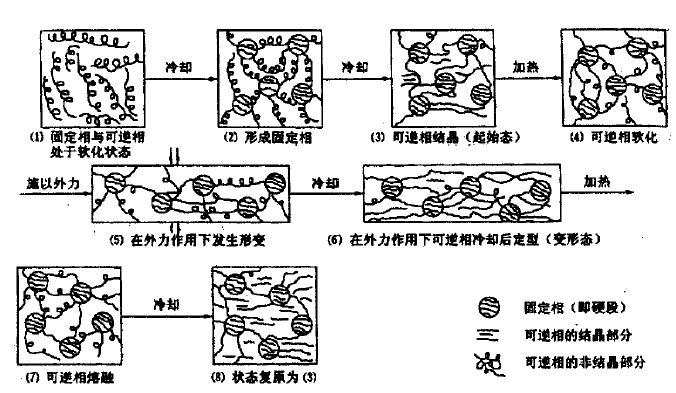
\includegraphics[width=0.75\textwidth]{chapters/chapter1/figures/figure1}
 \caption{热塑性形状记忆聚氨酯的形状记忆机理示意图}\label{fig:diagram}
\end{figure}


\subsection{形状记忆聚氨酯的研究进展}
%\label{sec:requirements}
首例SMPU是日本Mitsubishi公司开发成功的……。

\subsection{水系聚氨酯及聚氨酯整理剂}

水系聚氨酯的形态对其流动性,成膜性及加工织物的性能有重要影响,一般分为三种类型\cite{Jiang2005Size} ,如表 \ref{tab:category}所示。

\begin{table}
  \centering
  \caption{水系聚氨酯分类} \label{tab:category}
  \begin{tabular*}{0.9\textwidth}{@{\extracolsep{\fill}}cccc}
  \toprule
    类别			&水溶型		&胶体分散型		&乳液型 \\
  \midrule
    状态			&溶解$\sim$胶束	&分散		&白浊 \\
    外观			&水溶型		&胶体分散型		&乳液型 \\
    粒径$/\mu m$	&$<0.001$		&$0.001-0.1$		&$>0.1$ \\
    重均分子量	&$1000\sim 10000$	&数千$\sim 20万$ &$>5000$ \\
  \bottomrule
  \end{tabular*}
\end{table}

由于它们对纤维织物的浸透性和亲和性不同,因此在纺织品染整加工中的用途也有差别,其中以水溶型和乳液型产品较为常用。另外,水系聚氨酯又有反应性和非反应性之分。虽然它们的共同特点是分子结构中不含异氰酸酯基,但前者是用封闭剂将异氰酸酯基暂时封闭,在纺织品整理时复出。相互交联反应形成三维网状结构而固着在织物表面。
……



其他非顶层文件:\section{本论文研究的目的和意义}

近年来,随着人们生活水平的不断提高,人们越来越注重周围环境对身体健康的影响。作为服装是人们时时刻刻最贴近的环境,尤其是内衣,对人体健康有很大的影响。由于合时刻刻最贴近的环境,尤其是内衣,对人体健康有很大的影响。由于合成纤维的衣着舒适性、手感性,天然纤维的发展又成为人们关注的一大热点。

……\upcite{Takahashi1996Structure,Xia2002Analysis,Jiang1989,Mao2000Motion,Feng1998}
\end{lstlisting}

\section{与官方模板的区别}
\label{section:与官方模板的区别}
该模板基于官方v1.5版本修改,主要功能区别如下
\begin{enumerate}
\item 新增普通模式(normal)、自查重模式(selfSimilarCheck)和盲审模式(blindCheck)。提交学校的查重文件可以直接使用normal模式结果
;自查重模式主要用于关闭图片、公式等内容的显示,以减少文章字符数和降低PDF转word过程中出现的乱码,节省查重费用支出。应结合$\backslash$insertContents等系列命令使用。对于土豪此选项没有任何卵用。。。。。;盲审模式主要根据盲审文件格式要求,隐去了作者、导师、致谢等信息,更改发表论文的格式
\item 增加$\backslash$makeVerticalenWords命令,修改英文单词树立排放时的显示效果。
\item 增加书脊中作者姓名显示。
\item 增加对mathptmx包的引用,修改公式字体为New Time Roman。
\item{新增$\backslash$pubitem命令,用于显示学术成果。在盲审模式下该命令将会隐去作者信息。}
\item{新增$\backslash$sayThanks命令,用于致谢。在盲审模式下该命令指定的致谢内容将不被显示。}
\item{新增$\backslash$insertContents、$\backslash$insertFigure、$\backslash$insertTable、$\backslash$insertEquation系列指令,该指令用于自查重模式下选择性指定不显示的内容。}
\item{新增$\backslash$ncite、$\backslash$nupcite、$\backslash$nref命令,自查重模式下将不显示}
\item{修复了官方v1.5版本中文献引用标注显示的字号和颜色。}
\item{目录中章节标题取消加粗显示}
\item{打印中文信息的命令更改为$\backslash$makeChineseInfo}
\item{修改英文信息中下划线的长度。}
\end{enumerate}